% Auto-generated by the analysis pipeline — do not edit
% y > 0: Overreacts  |  y < 0: Underreacts
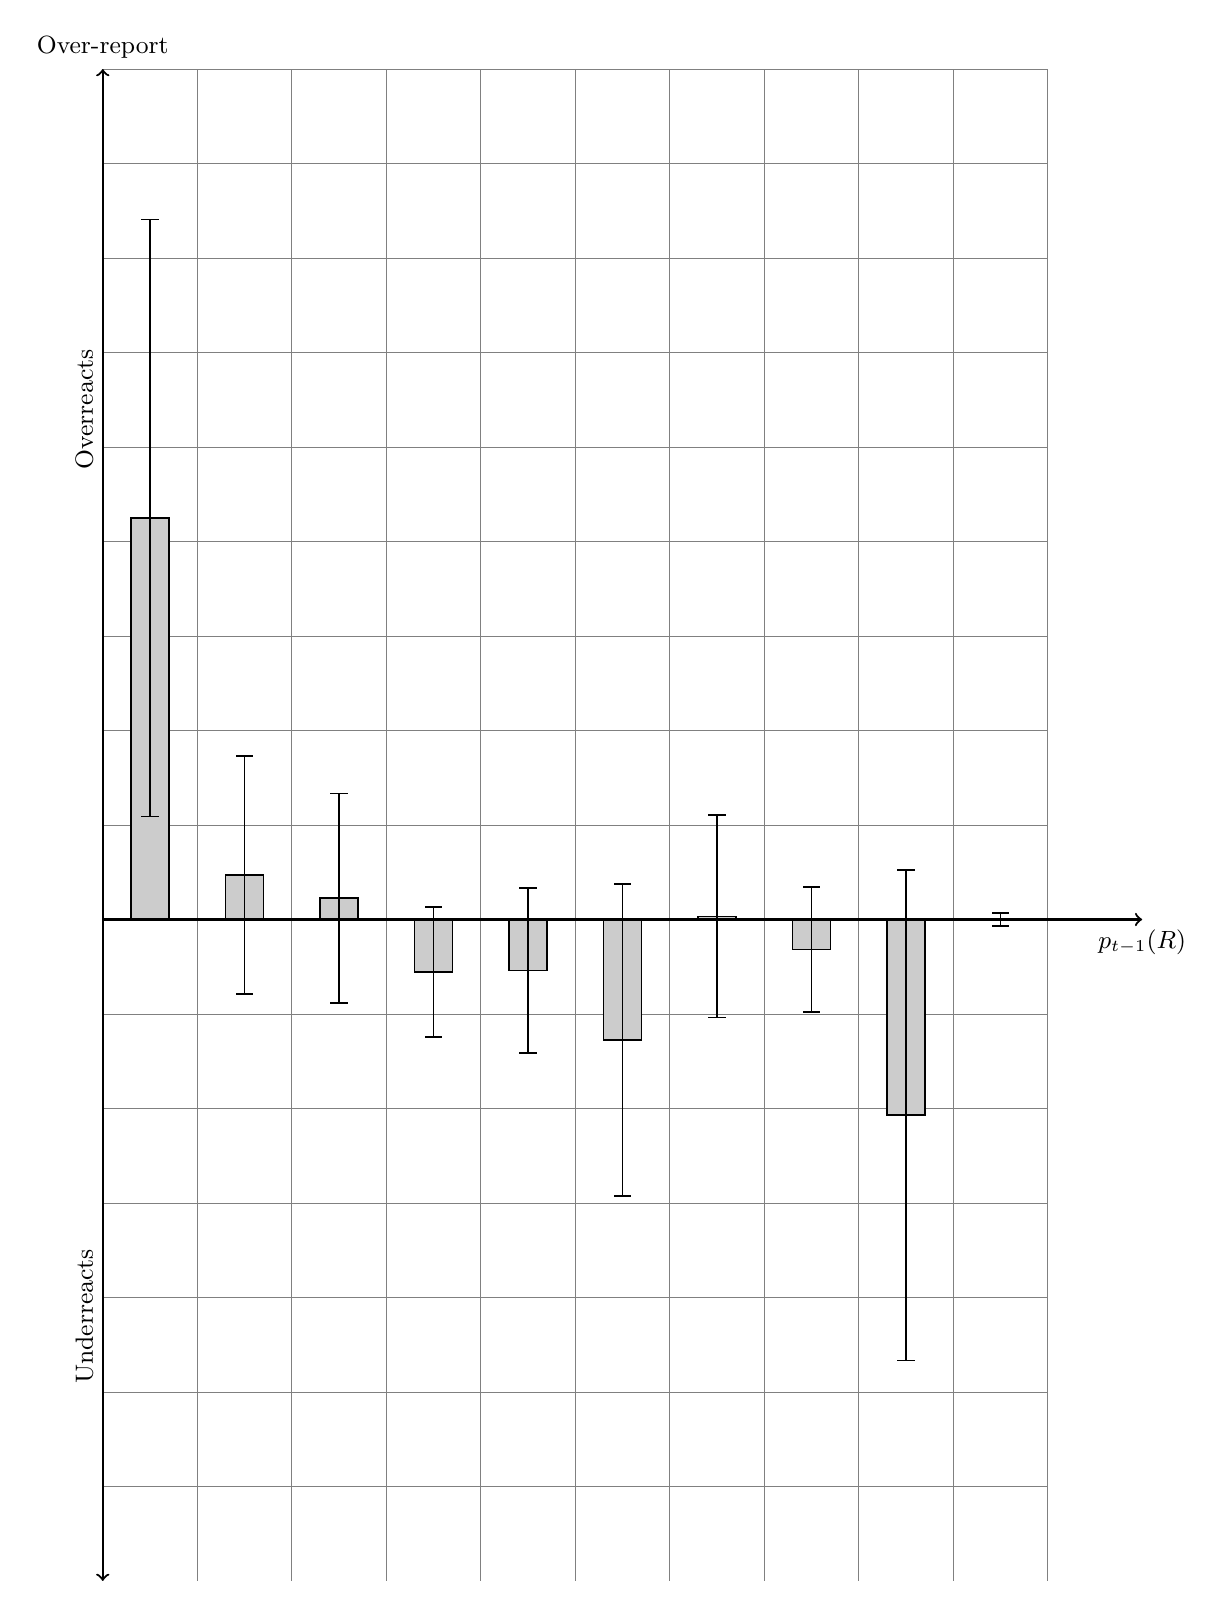
\begin{tikzpicture}[scale=12]
\draw[help lines,step=0.1] (0,-0.7) grid (1,0.9);
\filldraw[opaque,white!80!black] (0.03,0) rectangle (0.07,0.4250);
\draw[line width=0.6] (0.03,0) rectangle (0.07,0.4250);
\draw[line width=0.6,|-|] (0.05,0.1082) -- (0.05,0.7418);
\filldraw[opaque,white!80!black] (0.13,0) rectangle (0.17,0.0472);
\draw[line width=0.6] (0.13,0) rectangle (0.17,0.0472);
\draw[line width=0.6,|-|] (0.15,-0.0797) -- (0.15,0.1740);
\filldraw[opaque,white!80!black] (0.23,0) rectangle (0.27,0.0224);
\draw[line width=0.6] (0.23,0) rectangle (0.27,0.0224);
\draw[line width=0.6,|-|] (0.25,-0.0894) -- (0.25,0.1341);
\filldraw[opaque,white!80!black] (0.33,0) rectangle (0.37,-0.0558);
\draw[line width=0.6] (0.33,0) rectangle (0.37,-0.0558);
\draw[line width=0.6,|-|] (0.35,-0.1255) -- (0.35,0.0139);
\filldraw[opaque,white!80!black] (0.43,0) rectangle (0.47,-0.0539);
\draw[line width=0.6] (0.43,0) rectangle (0.47,-0.0539);
\draw[line width=0.6,|-|] (0.45,-0.1423) -- (0.45,0.0345);
\filldraw[opaque,white!80!black] (0.53,0) rectangle (0.57,-0.1275);
\draw[line width=0.6] (0.53,0) rectangle (0.57,-0.1275);
\draw[line width=0.6,|-|] (0.55,-0.2935) -- (0.55,0.0385);
\filldraw[opaque,white!80!black] (0.63,0) rectangle (0.67,0.0033);
\draw[line width=0.6] (0.63,0) rectangle (0.67,0.0033);
\draw[line width=0.6,|-|] (0.65,-0.1048) -- (0.65,0.1114);
\filldraw[opaque,white!80!black] (0.73,0) rectangle (0.77,-0.0317);
\draw[line width=0.6] (0.73,0) rectangle (0.77,-0.0317);
\draw[line width=0.6,|-|] (0.75,-0.0990) -- (0.75,0.0356);
\filldraw[opaque,white!80!black] (0.83,0) rectangle (0.87,-0.2072);
\draw[line width=0.6] (0.83,0) rectangle (0.87,-0.2072);
\draw[line width=0.6,|-|] (0.85,-0.4677) -- (0.85,0.0533);
\filldraw[opaque,white!80!black] (0.93,0) rectangle (0.97,-0.0001);
\draw[line width=0.6] (0.93,0) rectangle (0.97,-0.0001);
\draw[line width=0.6,|-|] (0.95,-0.0081) -- (0.95,0.0079);
\draw[line width=0.8,->]  (0,0) -- (1.1,0) node[below] {\small{$p_{t-1}(R)$}};
\draw[line width=0.8,<->] (0,-0.7) -- (0,0.9) node[above] {\small{Over-report}};
\draw (0,0.54) node[above,rotate=90] {\small{Overreacts}};
\draw (0,-0.42) node[above,rotate=90] {\small{Underreacts}};
% ADD THEORY CURVE BELOW
\end{tikzpicture}
